\documentclass[11pt]{article}
\usepackage[textwidth=18.0cm, textheight=23.0cm, top=2.0cm]{geometry}
\usepackage{pst-all}
\usepackage{amssymb}
\usepackage{tikz}
\usepackage{underscore}\begin{document}
\pagestyle{empty}


ClassName: \underline{\textbf{Class_03.2bp-17}}
\par
BinSize: \underline{\textbf{40 × 40}}
\par
ReduceSize: \underline{\textbf{40 × 40}}
\par
TypeNum: \underline{\textbf{40}}
\par
Num: \underline{\textbf{40}}
\par
OutS: \underline{\textbf{20800}}
\par
InS: \underline{\textbf{15902}}
\par
Rate: \underline{\textbf{0.765}}
\par
UB: \underline{\textbf{13}}
\par
LB0: \underline{\textbf{13}}
\par
LB: \underline{\textbf{13}}
\par
LBWithCut: \underline{\textbf{13}}
\par
NodeCut: \underline{\textbf{0}}
\par
ExtendedNodeCnt: \underline{\textbf{1}}
\par
GenNodeCnt: \underline{\textbf{1}}
\par
PrimalNode: \underline{\textbf{0}}
\par
ColumnCount: \underline{\textbf{13}}
\par
TotalCutCount: \underline{\textbf{0}}
\par
RootCutCount: \underline{\textbf{0}}
\par
LPSolverCnt: \underline{\textbf{1}}
\par
PricingSolverCnt: \underline{\textbf{0}}
\par
BranchAndBoundNum: \underline{\textbf{1}}
\par
isOpt: \underline{\textbf{true}}
\par
TimeOnPrimal: \underline{\textbf{0.000 s}}
\par
TimeOnPricing: \underline{\textbf{0.000 s}}
\par
TimeOnRmp: \underline{\textbf{0.062 s}}
\par
TotalTime: \underline{\textbf{0.125 s}}
\par
\newpage


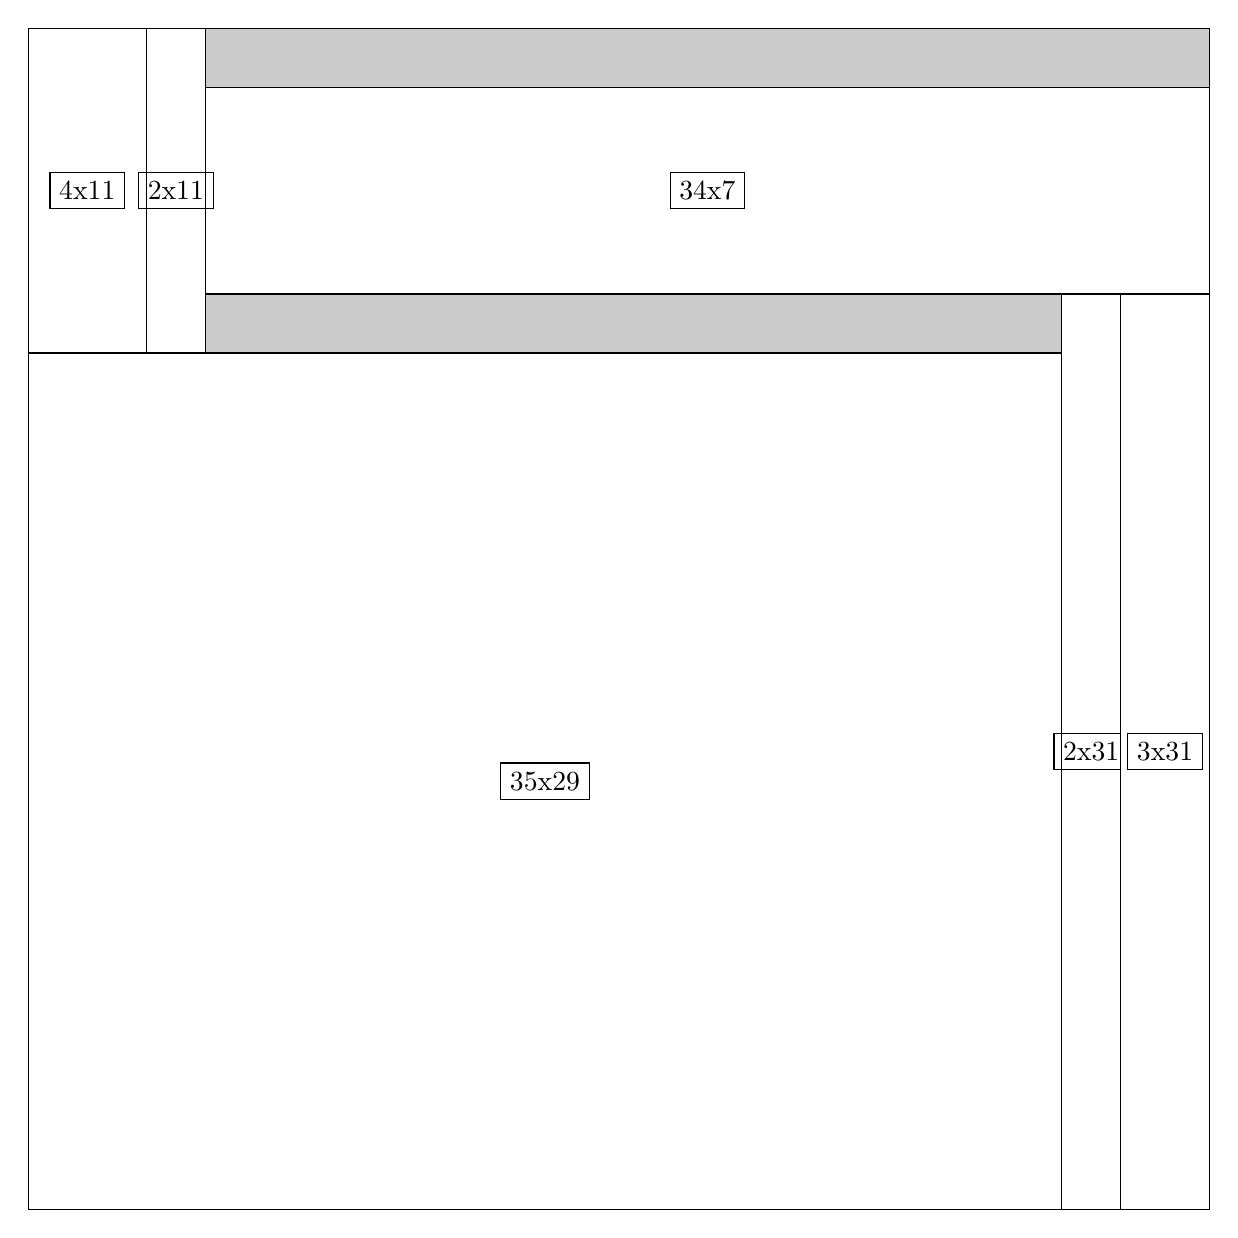
\begin{tikzpicture}[shorten >=1pt,scale=1.0,every node/.style={scale=1.0},->]
\tikzstyle{vertex}=[circle,fill=black!25,minimum size=14pt,inner sep=0pt]
\filldraw[fill=gray!40!white, draw=black] (0,0) rectangle (15.0,15.0);
\foreach \name/\x/\y/\w/\h in {35x29/0.0/0.0/13.125/10.875,2x31/13.125/0.0/0.75/11.625,3x31/13.875/0.0/1.125/11.625,34x7/2.25/11.625/12.75/2.625,4x11/0.0/10.875/1.5/4.125,2x11/1.5/10.875/0.75/4.125}
\filldraw[fill=white!40!white, draw=black] (\x,\y) rectangle node[draw] (\name) {\name} ++(\w,\h);
\end{tikzpicture}


w =35 , h =29 , x =0 , y =0 , v =1015
\par
w =2 , h =31 , x =35 , y =0 , v =62
\par
w =3 , h =31 , x =37 , y =0 , v =93
\par
w =34 , h =7 , x =6 , y =31 , v =238
\par
w =4 , h =11 , x =0 , y =29 , v =44
\par
w =2 , h =11 , x =4 , y =29 , v =22
\par
\newpage


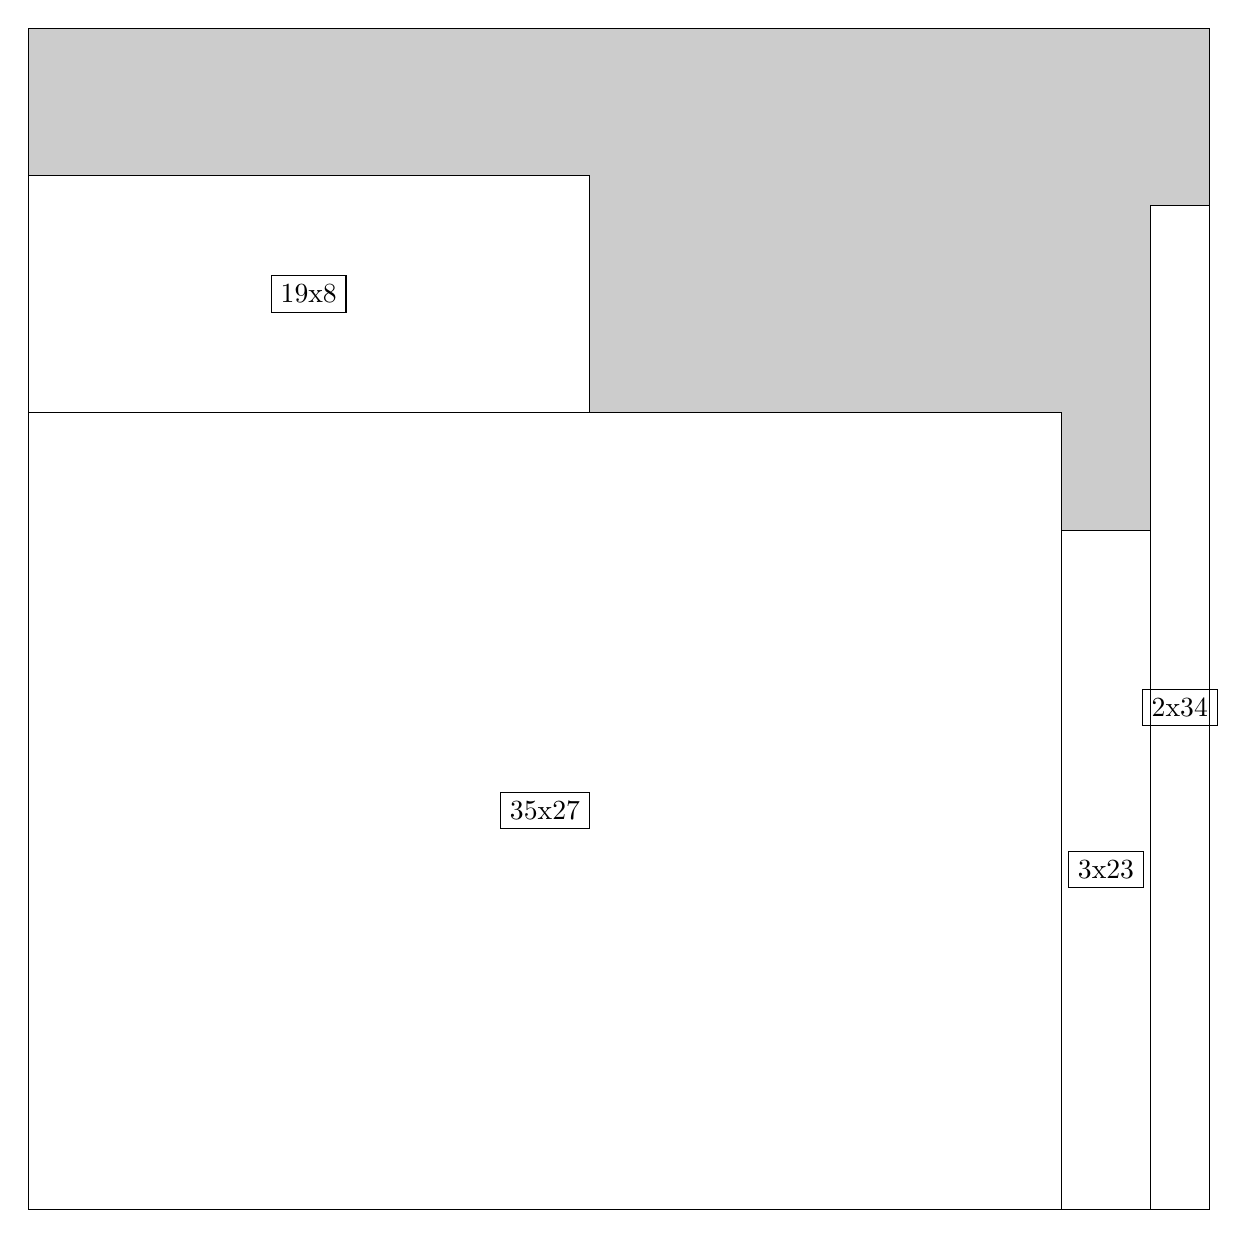
\begin{tikzpicture}[shorten >=1pt,scale=1.0,every node/.style={scale=1.0},->]
\tikzstyle{vertex}=[circle,fill=black!25,minimum size=14pt,inner sep=0pt]
\filldraw[fill=gray!40!white, draw=black] (0,0) rectangle (15.0,15.0);
\foreach \name/\x/\y/\w/\h in {35x27/0.0/0.0/13.125/10.125,19x8/0.0/10.125/7.125/3.0,3x23/13.125/0.0/1.125/8.625,2x34/14.25/0.0/0.75/12.75}
\filldraw[fill=white!40!white, draw=black] (\x,\y) rectangle node[draw] (\name) {\name} ++(\w,\h);
\end{tikzpicture}


w =35 , h =27 , x =0 , y =0 , v =945
\par
w =19 , h =8 , x =0 , y =27 , v =152
\par
w =3 , h =23 , x =35 , y =0 , v =69
\par
w =2 , h =34 , x =38 , y =0 , v =68
\par
\newpage


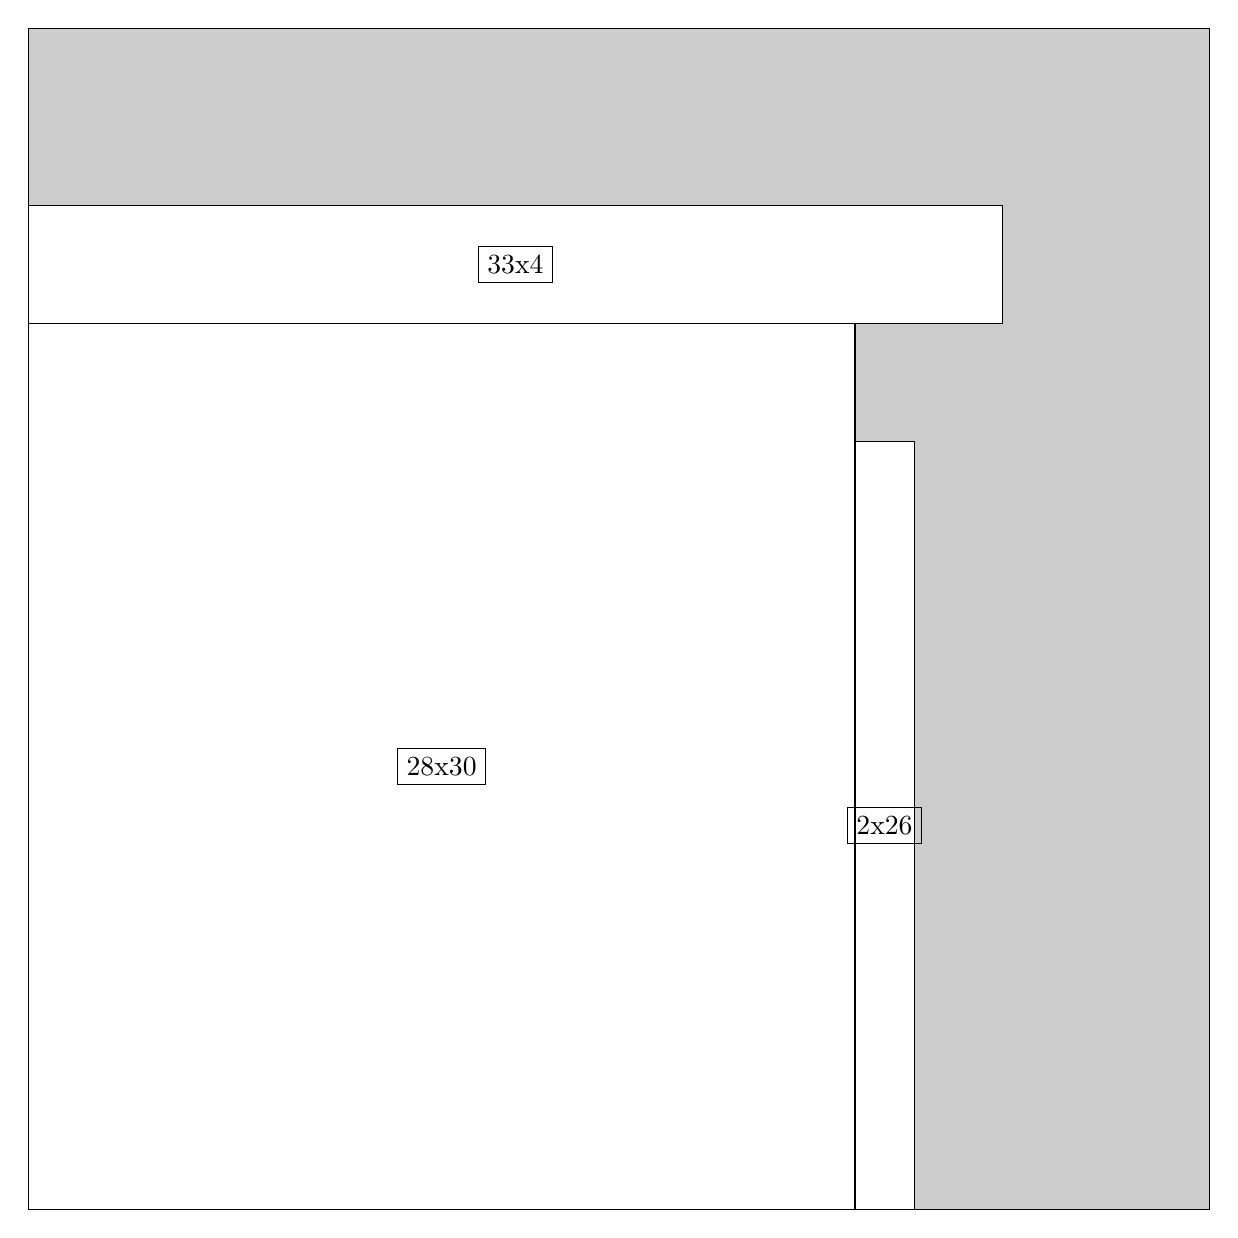
\begin{tikzpicture}[shorten >=1pt,scale=1.0,every node/.style={scale=1.0},->]
\tikzstyle{vertex}=[circle,fill=black!25,minimum size=14pt,inner sep=0pt]
\filldraw[fill=gray!40!white, draw=black] (0,0) rectangle (15.0,15.0);
\foreach \name/\x/\y/\w/\h in {28x30/0.0/0.0/10.5/11.25,33x4/0.0/11.25/12.375/1.5,2x26/10.5/0.0/0.75/9.75}
\filldraw[fill=white!40!white, draw=black] (\x,\y) rectangle node[draw] (\name) {\name} ++(\w,\h);
\end{tikzpicture}


w =28 , h =30 , x =0 , y =0 , v =840
\par
w =33 , h =4 , x =0 , y =30 , v =132
\par
w =2 , h =26 , x =28 , y =0 , v =52
\par
\newpage


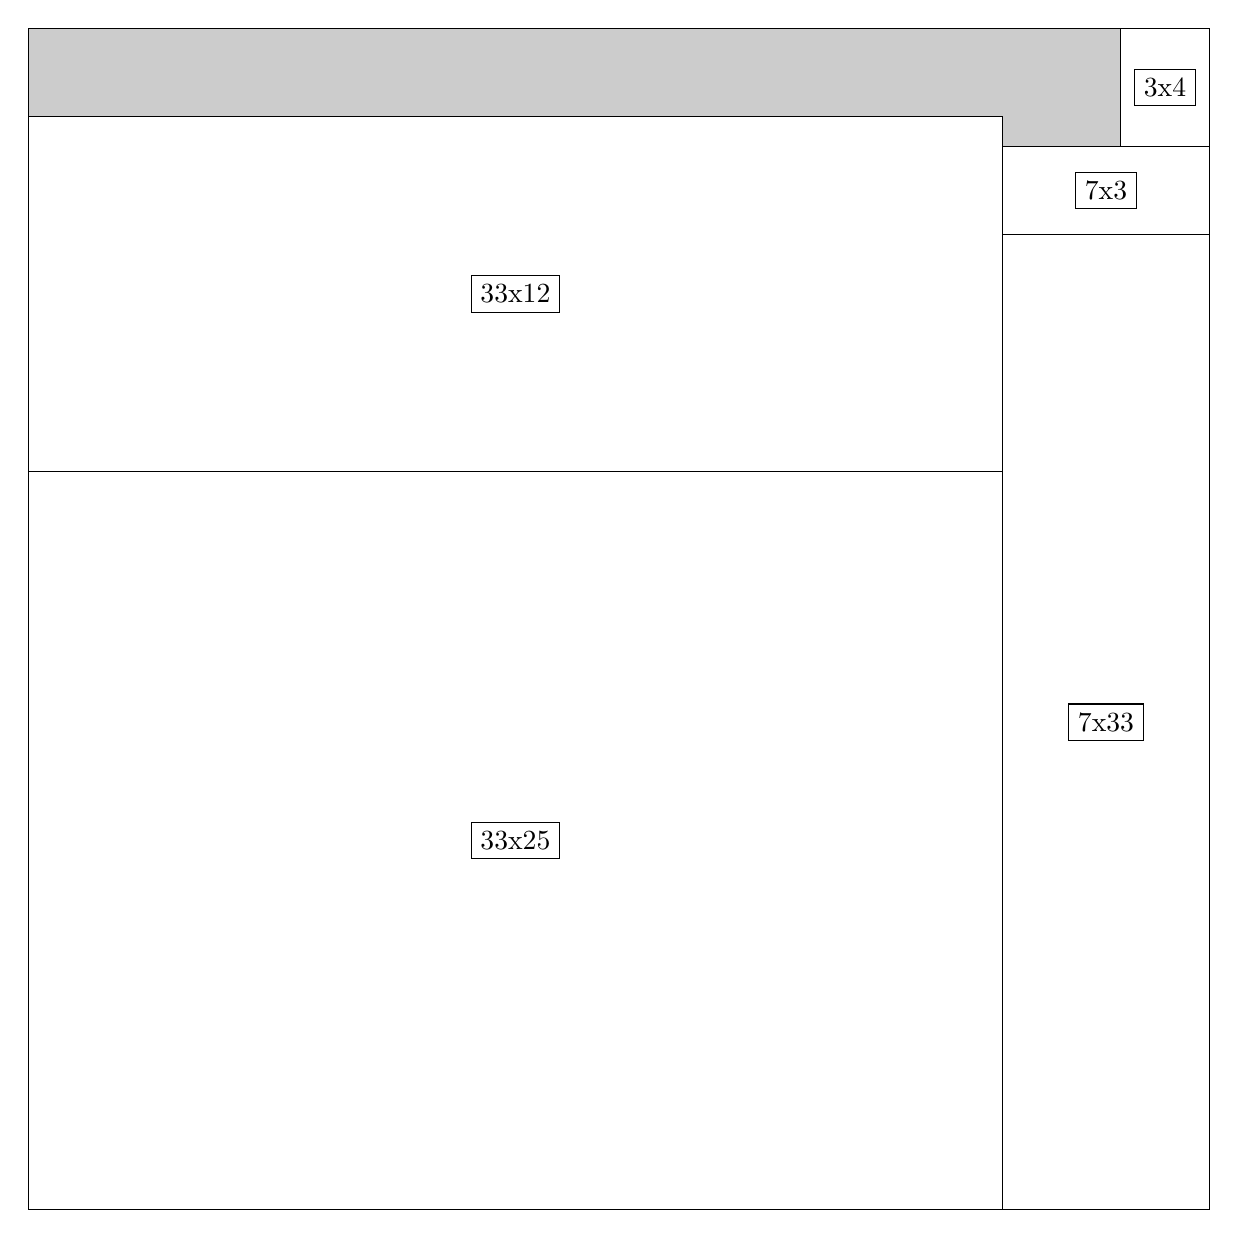
\begin{tikzpicture}[shorten >=1pt,scale=1.0,every node/.style={scale=1.0},->]
\tikzstyle{vertex}=[circle,fill=black!25,minimum size=14pt,inner sep=0pt]
\filldraw[fill=gray!40!white, draw=black] (0,0) rectangle (15.0,15.0);
\foreach \name/\x/\y/\w/\h in {33x25/0.0/0.0/12.375/9.375,33x12/0.0/9.375/12.375/4.5,7x33/12.375/0.0/2.625/12.375,7x3/12.375/12.375/2.625/1.125,3x4/13.875/13.5/1.125/1.5}
\filldraw[fill=white!40!white, draw=black] (\x,\y) rectangle node[draw] (\name) {\name} ++(\w,\h);
\end{tikzpicture}


w =33 , h =25 , x =0 , y =0 , v =825
\par
w =33 , h =12 , x =0 , y =25 , v =396
\par
w =7 , h =33 , x =33 , y =0 , v =231
\par
w =7 , h =3 , x =33 , y =33 , v =21
\par
w =3 , h =4 , x =37 , y =36 , v =12
\par
\newpage


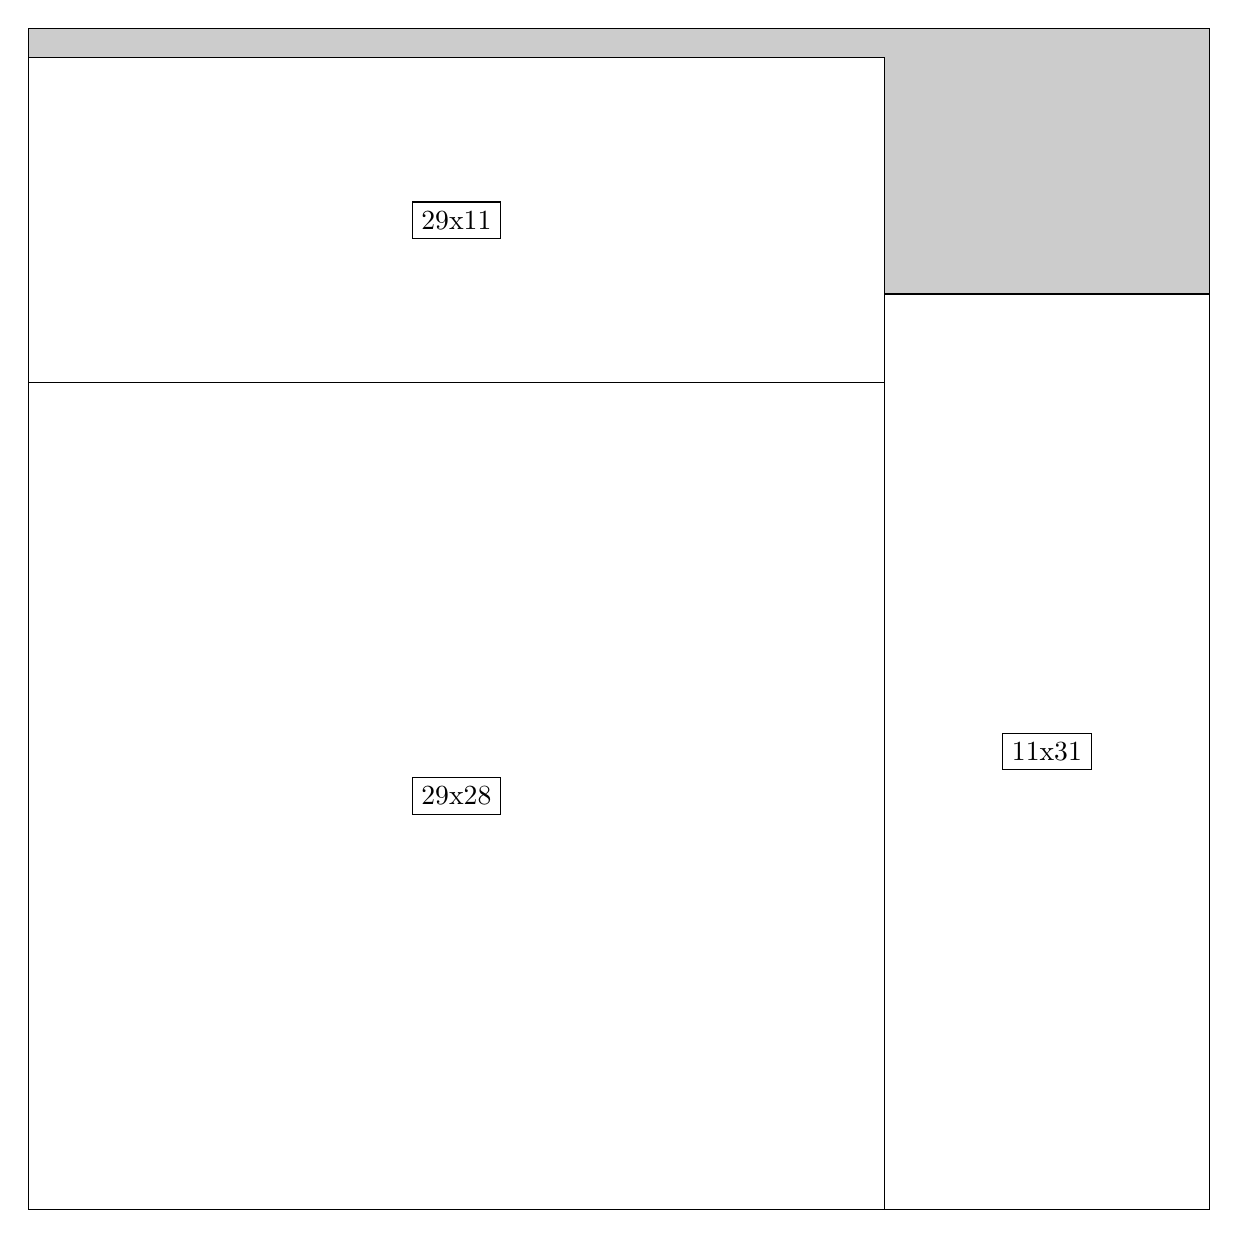
\begin{tikzpicture}[shorten >=1pt,scale=1.0,every node/.style={scale=1.0},->]
\tikzstyle{vertex}=[circle,fill=black!25,minimum size=14pt,inner sep=0pt]
\filldraw[fill=gray!40!white, draw=black] (0,0) rectangle (15.0,15.0);
\foreach \name/\x/\y/\w/\h in {29x28/0.0/0.0/10.875/10.5,11x31/10.875/0.0/4.125/11.625,29x11/0.0/10.5/10.875/4.125}
\filldraw[fill=white!40!white, draw=black] (\x,\y) rectangle node[draw] (\name) {\name} ++(\w,\h);
\end{tikzpicture}


w =29 , h =28 , x =0 , y =0 , v =812
\par
w =11 , h =31 , x =29 , y =0 , v =341
\par
w =29 , h =11 , x =0 , y =28 , v =319
\par
\newpage


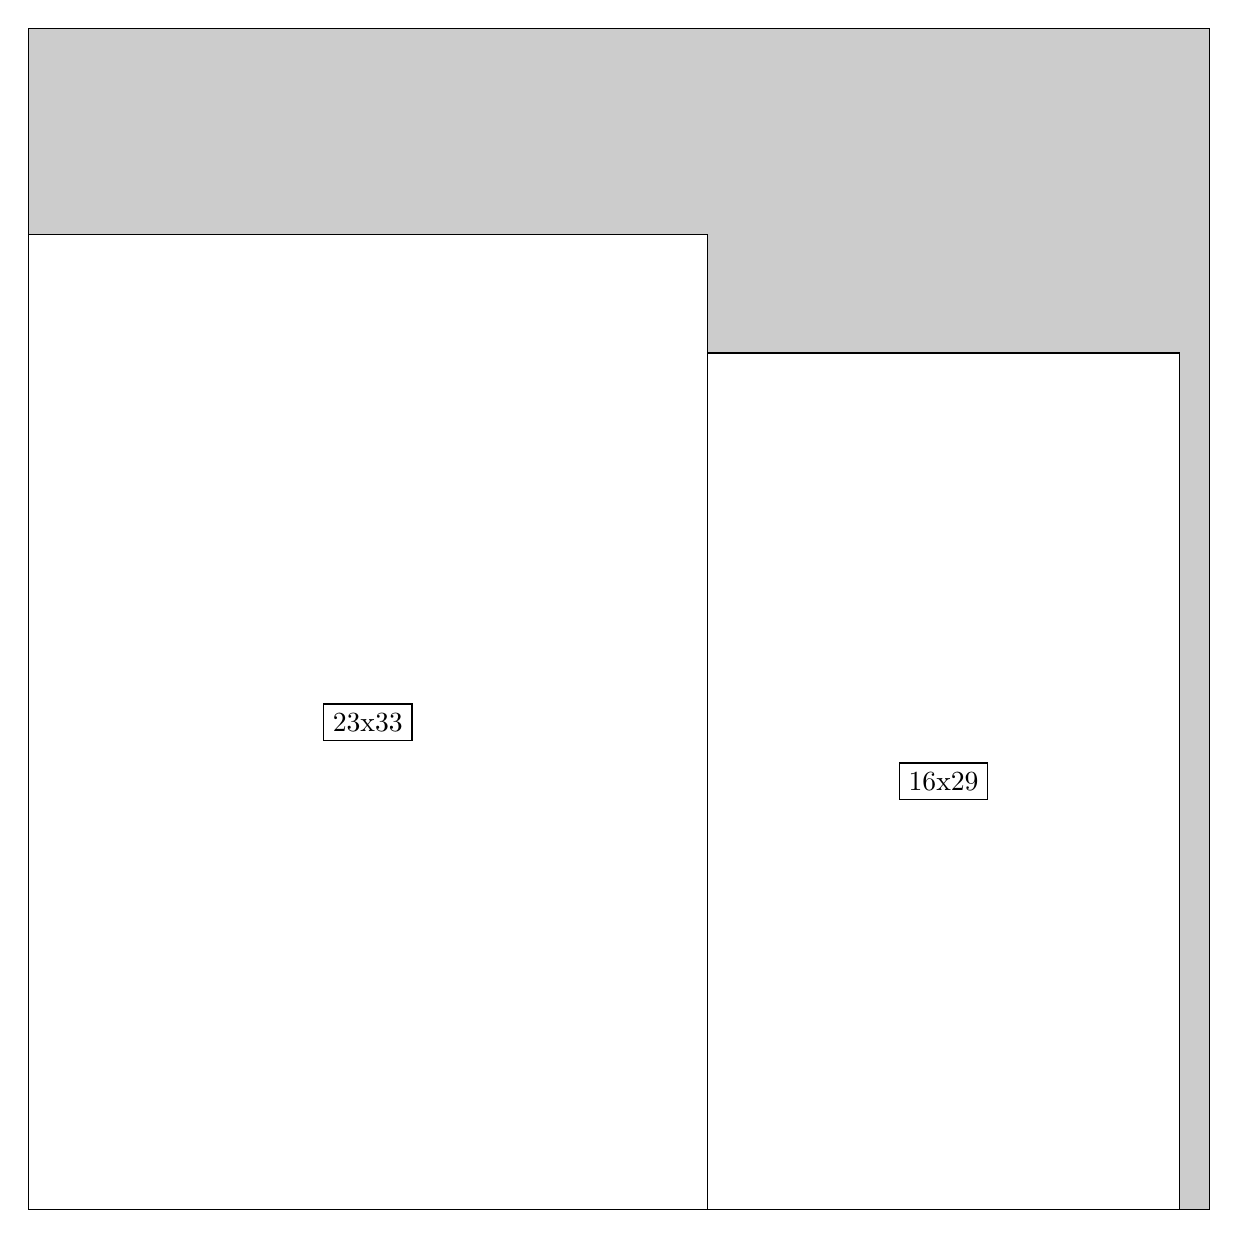
\begin{tikzpicture}[shorten >=1pt,scale=1.0,every node/.style={scale=1.0},->]
\tikzstyle{vertex}=[circle,fill=black!25,minimum size=14pt,inner sep=0pt]
\filldraw[fill=gray!40!white, draw=black] (0,0) rectangle (15.0,15.0);
\foreach \name/\x/\y/\w/\h in {23x33/0.0/0.0/8.625/12.375,16x29/8.625/0.0/6.0/10.875}
\filldraw[fill=white!40!white, draw=black] (\x,\y) rectangle node[draw] (\name) {\name} ++(\w,\h);
\end{tikzpicture}


w =23 , h =33 , x =0 , y =0 , v =759
\par
w =16 , h =29 , x =23 , y =0 , v =464
\par
\newpage


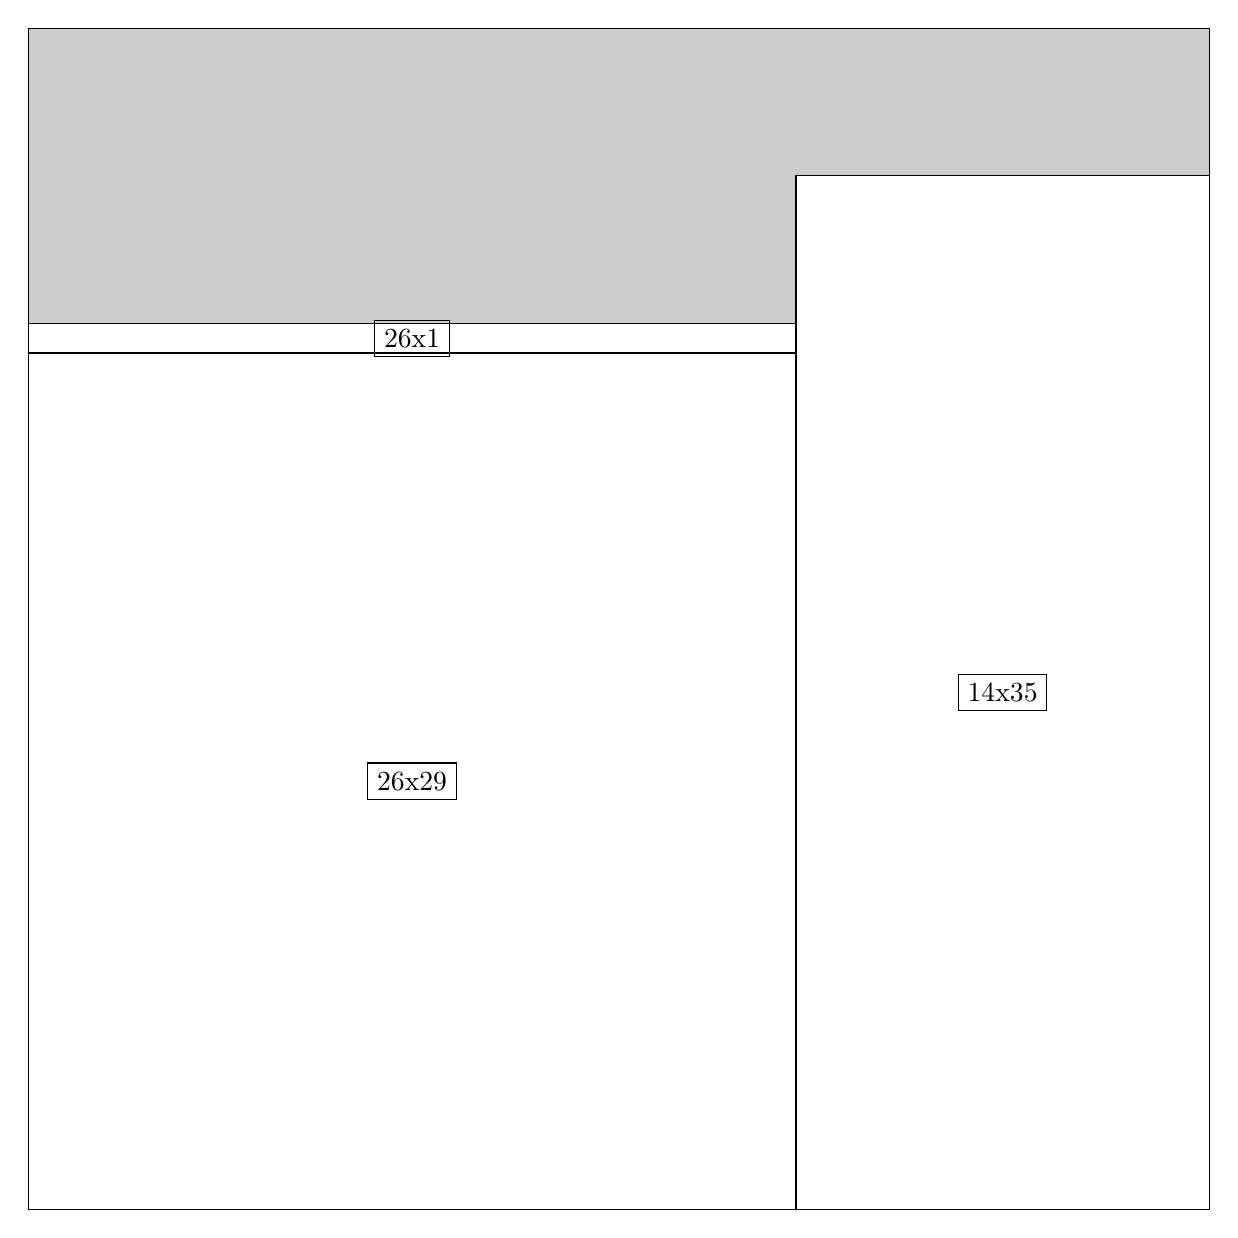
\begin{tikzpicture}[shorten >=1pt,scale=1.0,every node/.style={scale=1.0},->]
\tikzstyle{vertex}=[circle,fill=black!25,minimum size=14pt,inner sep=0pt]
\filldraw[fill=gray!40!white, draw=black] (0,0) rectangle (15.0,15.0);
\foreach \name/\x/\y/\w/\h in {26x29/0.0/0.0/9.75/10.875,14x35/9.75/0.0/5.25/13.125,26x1/0.0/10.875/9.75/0.375}
\filldraw[fill=white!40!white, draw=black] (\x,\y) rectangle node[draw] (\name) {\name} ++(\w,\h);
\end{tikzpicture}


w =26 , h =29 , x =0 , y =0 , v =754
\par
w =14 , h =35 , x =26 , y =0 , v =490
\par
w =26 , h =1 , x =0 , y =29 , v =26
\par
\newpage


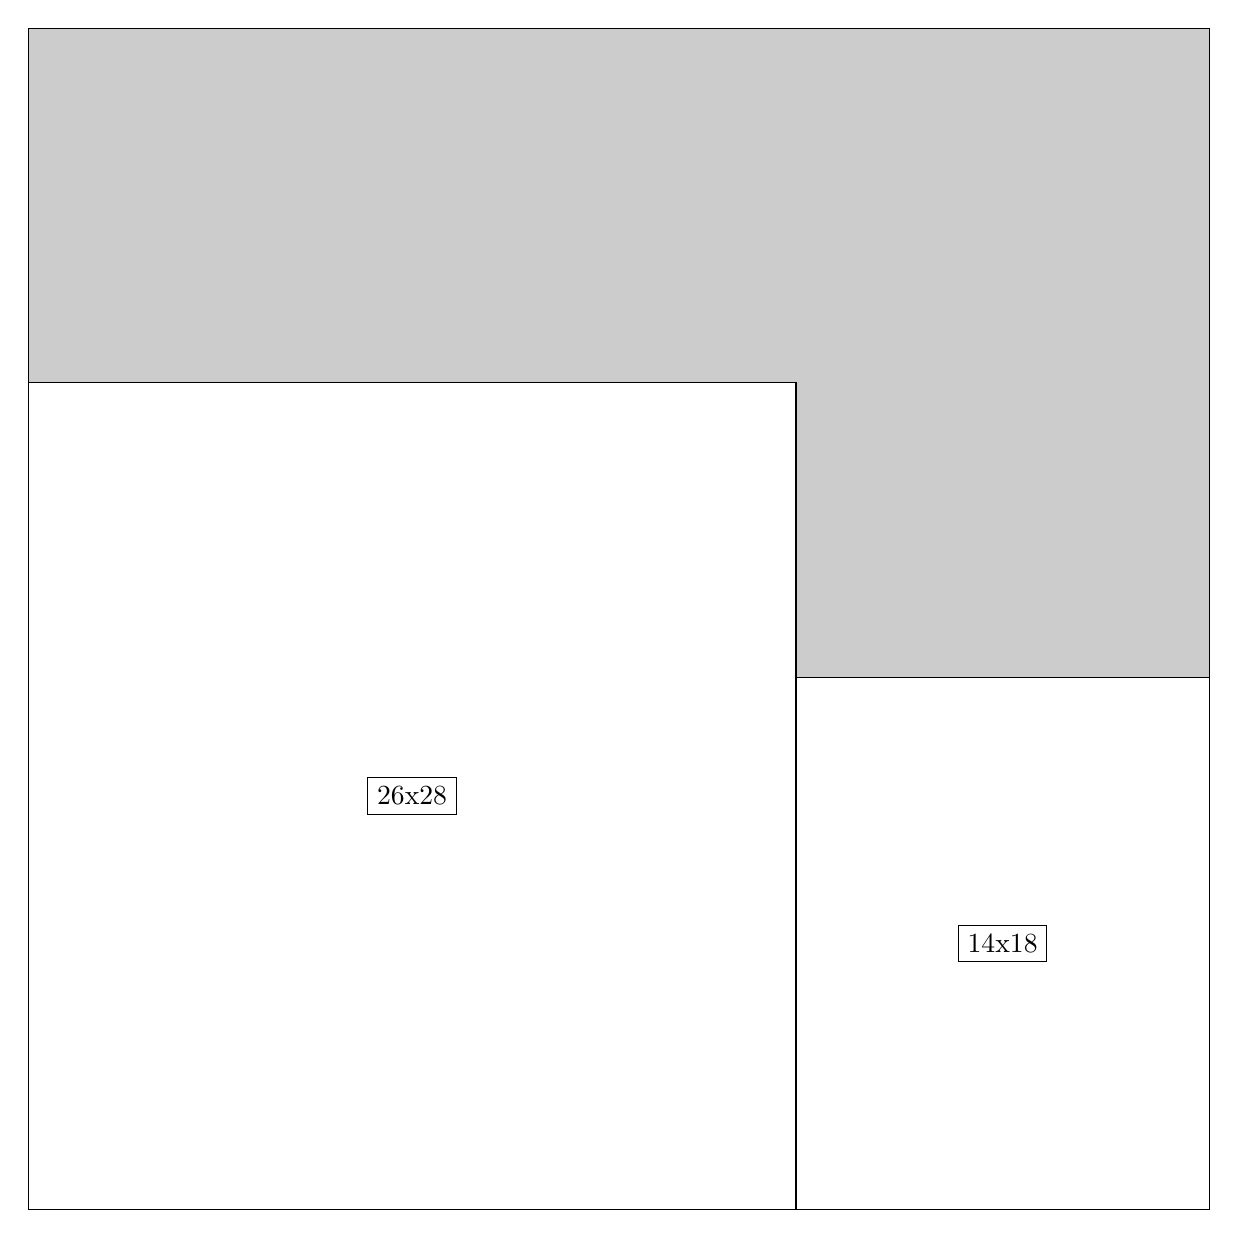
\begin{tikzpicture}[shorten >=1pt,scale=1.0,every node/.style={scale=1.0},->]
\tikzstyle{vertex}=[circle,fill=black!25,minimum size=14pt,inner sep=0pt]
\filldraw[fill=gray!40!white, draw=black] (0,0) rectangle (15.0,15.0);
\foreach \name/\x/\y/\w/\h in {26x28/0.0/0.0/9.75/10.5,14x18/9.75/0.0/5.25/6.75}
\filldraw[fill=white!40!white, draw=black] (\x,\y) rectangle node[draw] (\name) {\name} ++(\w,\h);
\end{tikzpicture}


w =26 , h =28 , x =0 , y =0 , v =728
\par
w =14 , h =18 , x =26 , y =0 , v =252
\par
\newpage


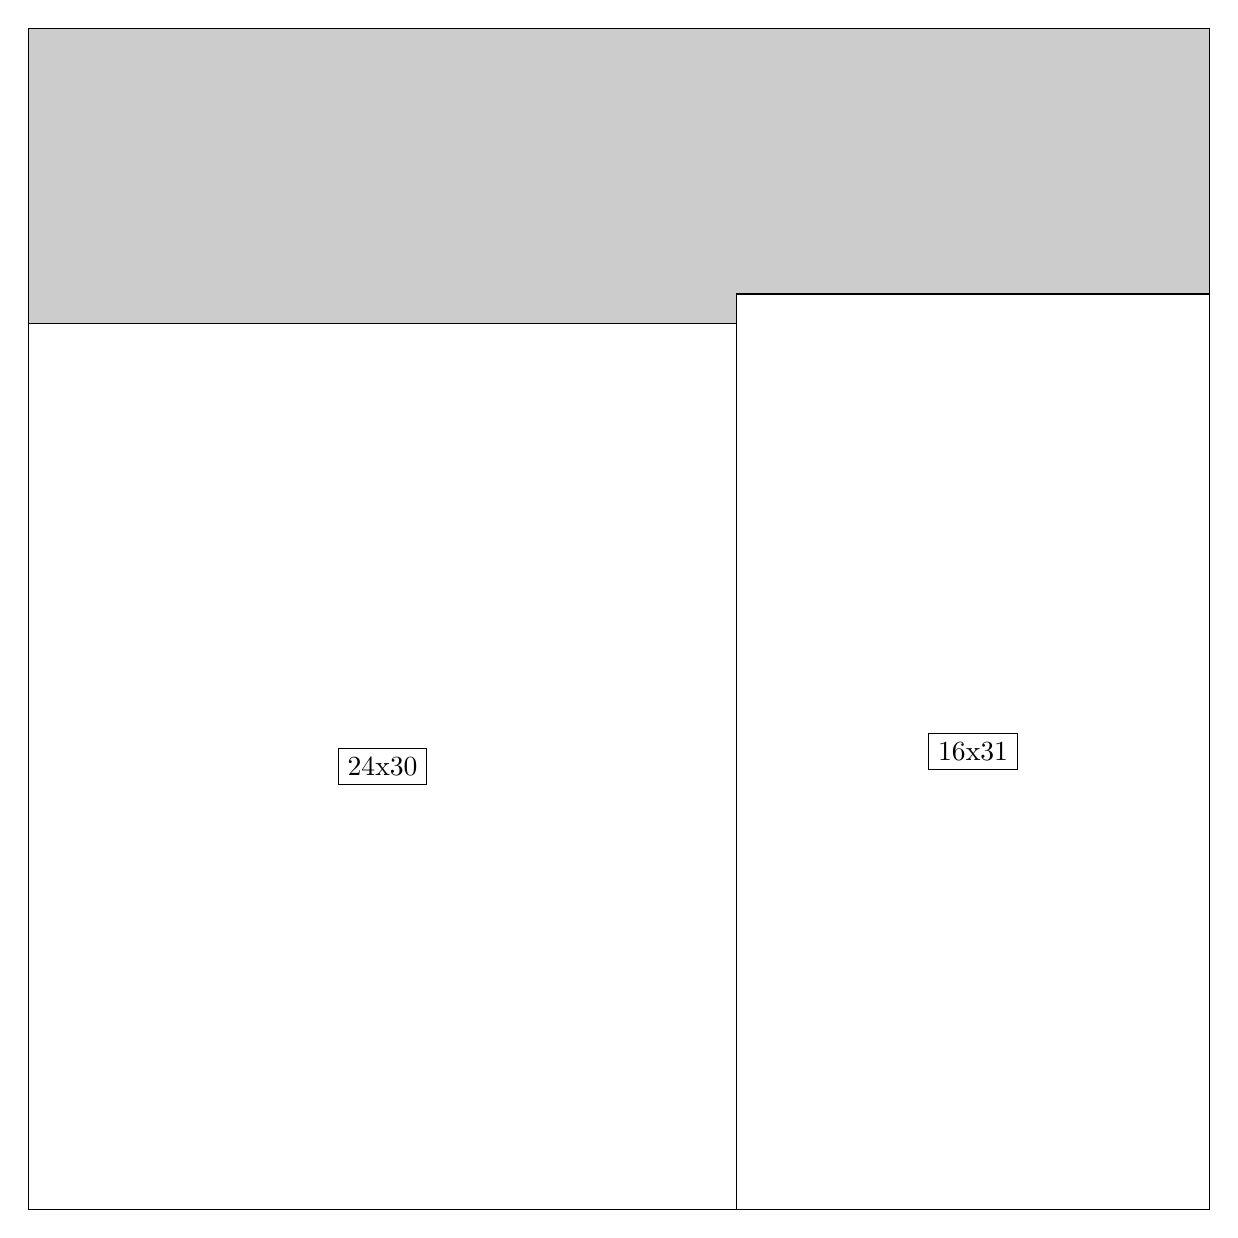
\begin{tikzpicture}[shorten >=1pt,scale=1.0,every node/.style={scale=1.0},->]
\tikzstyle{vertex}=[circle,fill=black!25,minimum size=14pt,inner sep=0pt]
\filldraw[fill=gray!40!white, draw=black] (0,0) rectangle (15.0,15.0);
\foreach \name/\x/\y/\w/\h in {24x30/0.0/0.0/9.0/11.25,16x31/9.0/0.0/6.0/11.625}
\filldraw[fill=white!40!white, draw=black] (\x,\y) rectangle node[draw] (\name) {\name} ++(\w,\h);
\end{tikzpicture}


w =24 , h =30 , x =0 , y =0 , v =720
\par
w =16 , h =31 , x =24 , y =0 , v =496
\par
\newpage


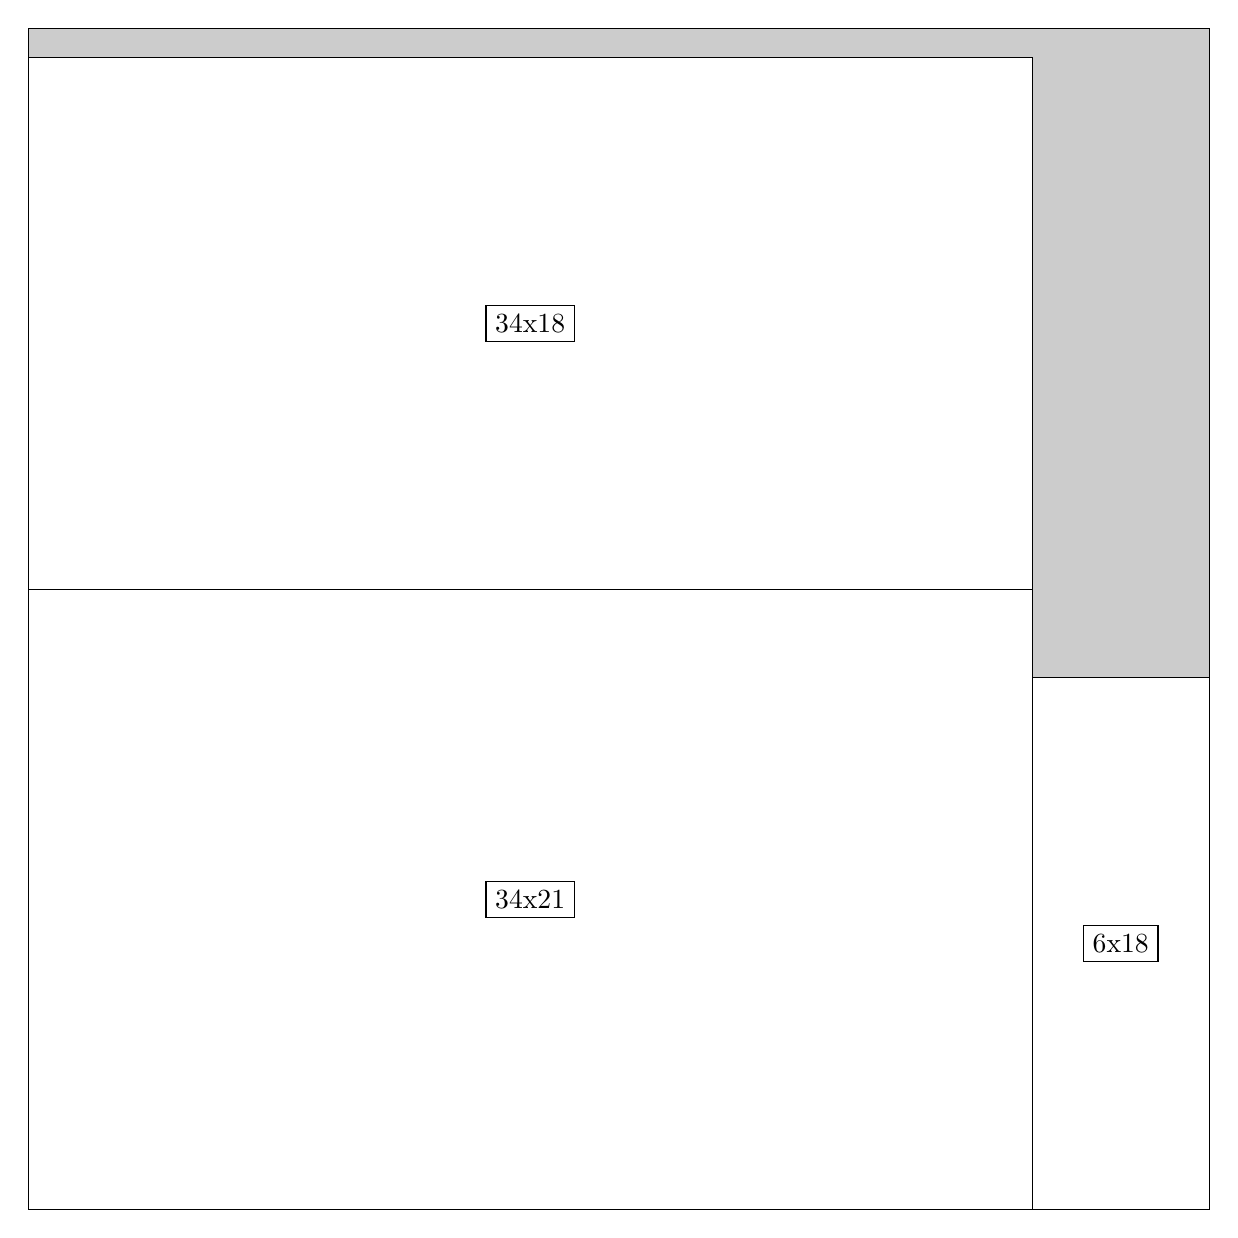
\begin{tikzpicture}[shorten >=1pt,scale=1.0,every node/.style={scale=1.0},->]
\tikzstyle{vertex}=[circle,fill=black!25,minimum size=14pt,inner sep=0pt]
\filldraw[fill=gray!40!white, draw=black] (0,0) rectangle (15.0,15.0);
\foreach \name/\x/\y/\w/\h in {34x21/0.0/0.0/12.75/7.875,34x18/0.0/7.875/12.75/6.75,6x18/12.75/0.0/2.25/6.75}
\filldraw[fill=white!40!white, draw=black] (\x,\y) rectangle node[draw] (\name) {\name} ++(\w,\h);
\end{tikzpicture}


w =34 , h =21 , x =0 , y =0 , v =714
\par
w =34 , h =18 , x =0 , y =21 , v =612
\par
w =6 , h =18 , x =34 , y =0 , v =108
\par
\newpage


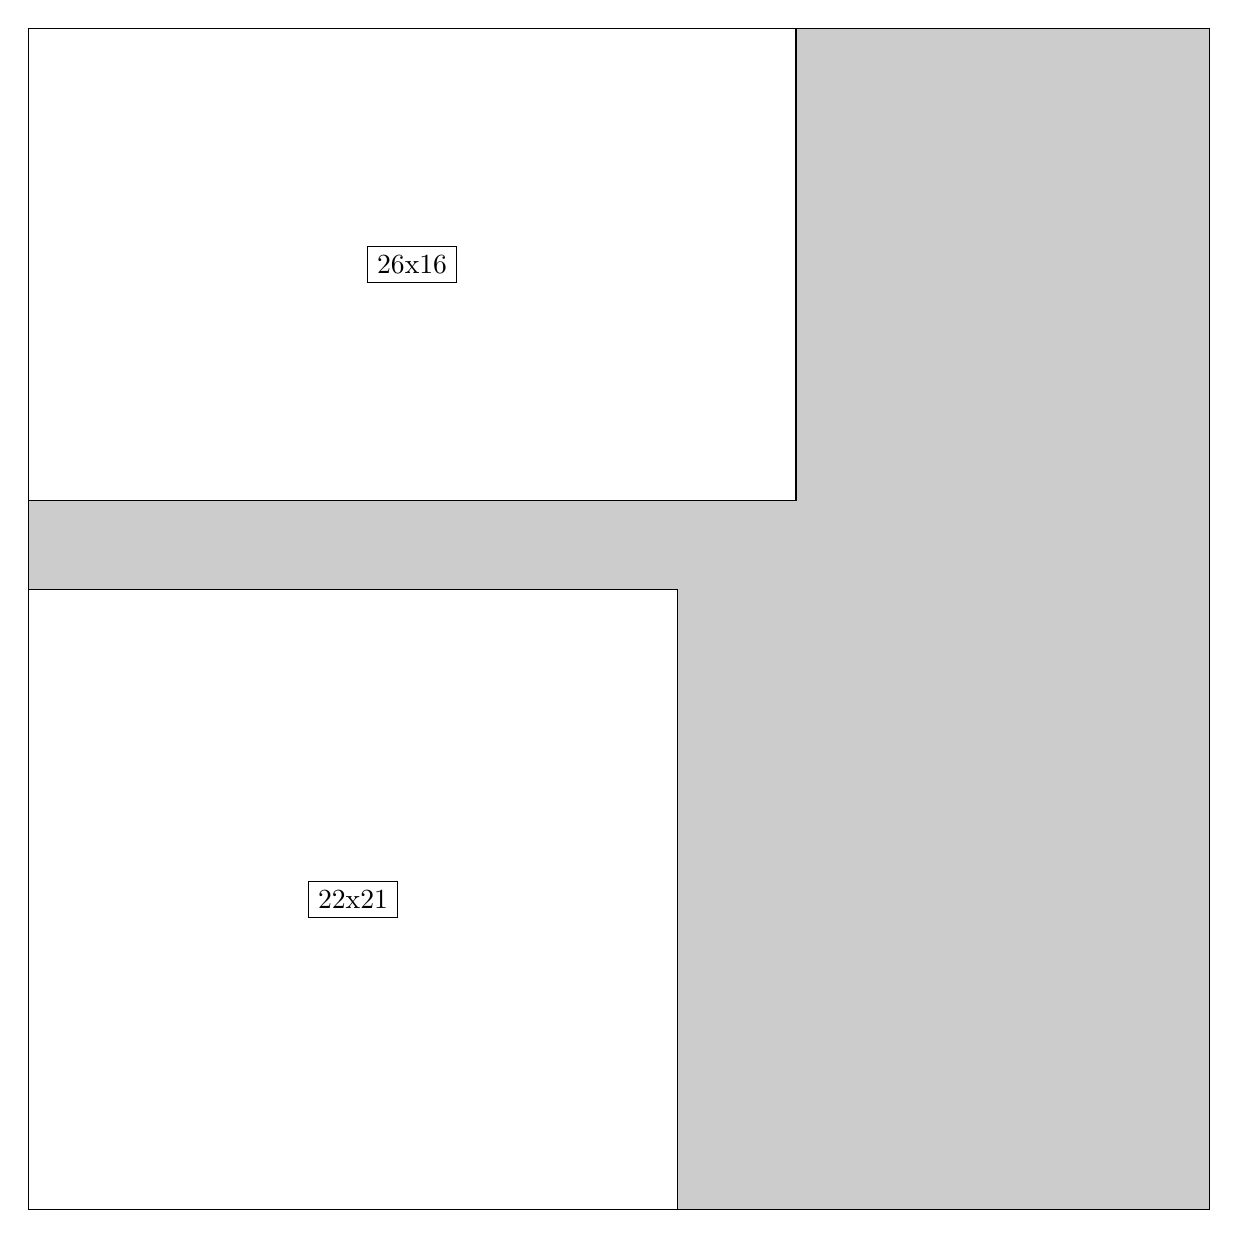
\begin{tikzpicture}[shorten >=1pt,scale=1.0,every node/.style={scale=1.0},->]
\tikzstyle{vertex}=[circle,fill=black!25,minimum size=14pt,inner sep=0pt]
\filldraw[fill=gray!40!white, draw=black] (0,0) rectangle (15.0,15.0);
\foreach \name/\x/\y/\w/\h in {22x21/0.0/0.0/8.25/7.875,26x16/0.0/9.0/9.75/6.0}
\filldraw[fill=white!40!white, draw=black] (\x,\y) rectangle node[draw] (\name) {\name} ++(\w,\h);
\end{tikzpicture}


w =22 , h =21 , x =0 , y =0 , v =462
\par
w =26 , h =16 , x =0 , y =24 , v =416
\par
\newpage


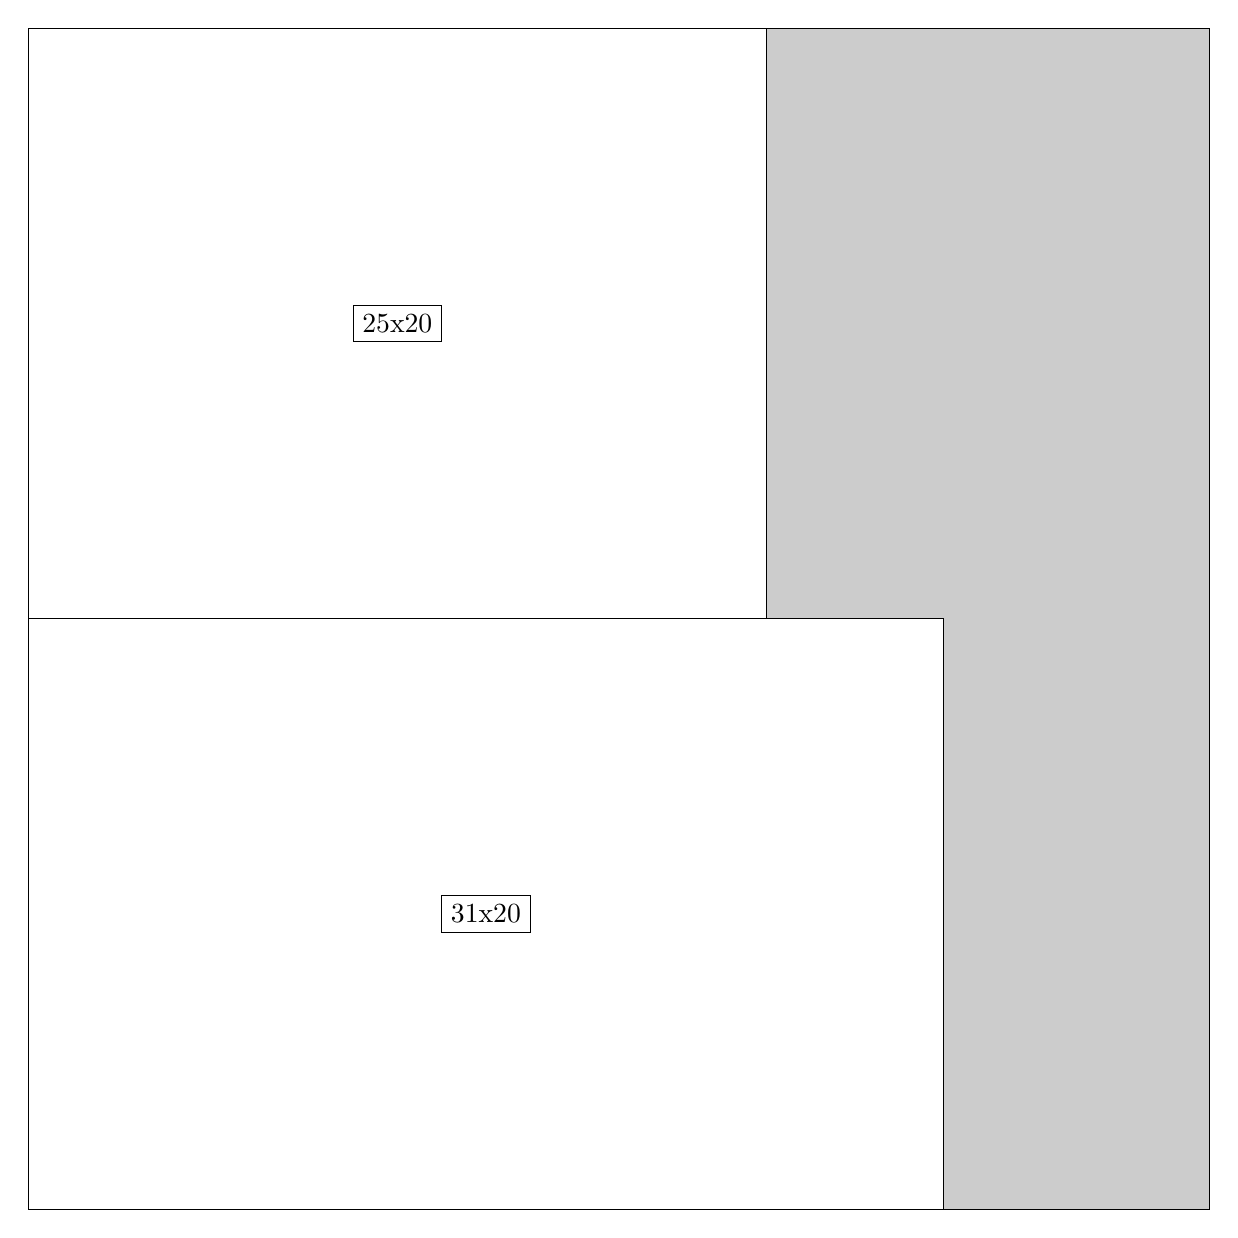
\begin{tikzpicture}[shorten >=1pt,scale=1.0,every node/.style={scale=1.0},->]
\tikzstyle{vertex}=[circle,fill=black!25,minimum size=14pt,inner sep=0pt]
\filldraw[fill=gray!40!white, draw=black] (0,0) rectangle (15.0,15.0);
\foreach \name/\x/\y/\w/\h in {31x20/0.0/0.0/11.625/7.5,25x20/0.0/7.5/9.375/7.5}
\filldraw[fill=white!40!white, draw=black] (\x,\y) rectangle node[draw] (\name) {\name} ++(\w,\h);
\end{tikzpicture}


w =31 , h =20 , x =0 , y =0 , v =620
\par
w =25 , h =20 , x =0 , y =20 , v =500
\par
\newpage


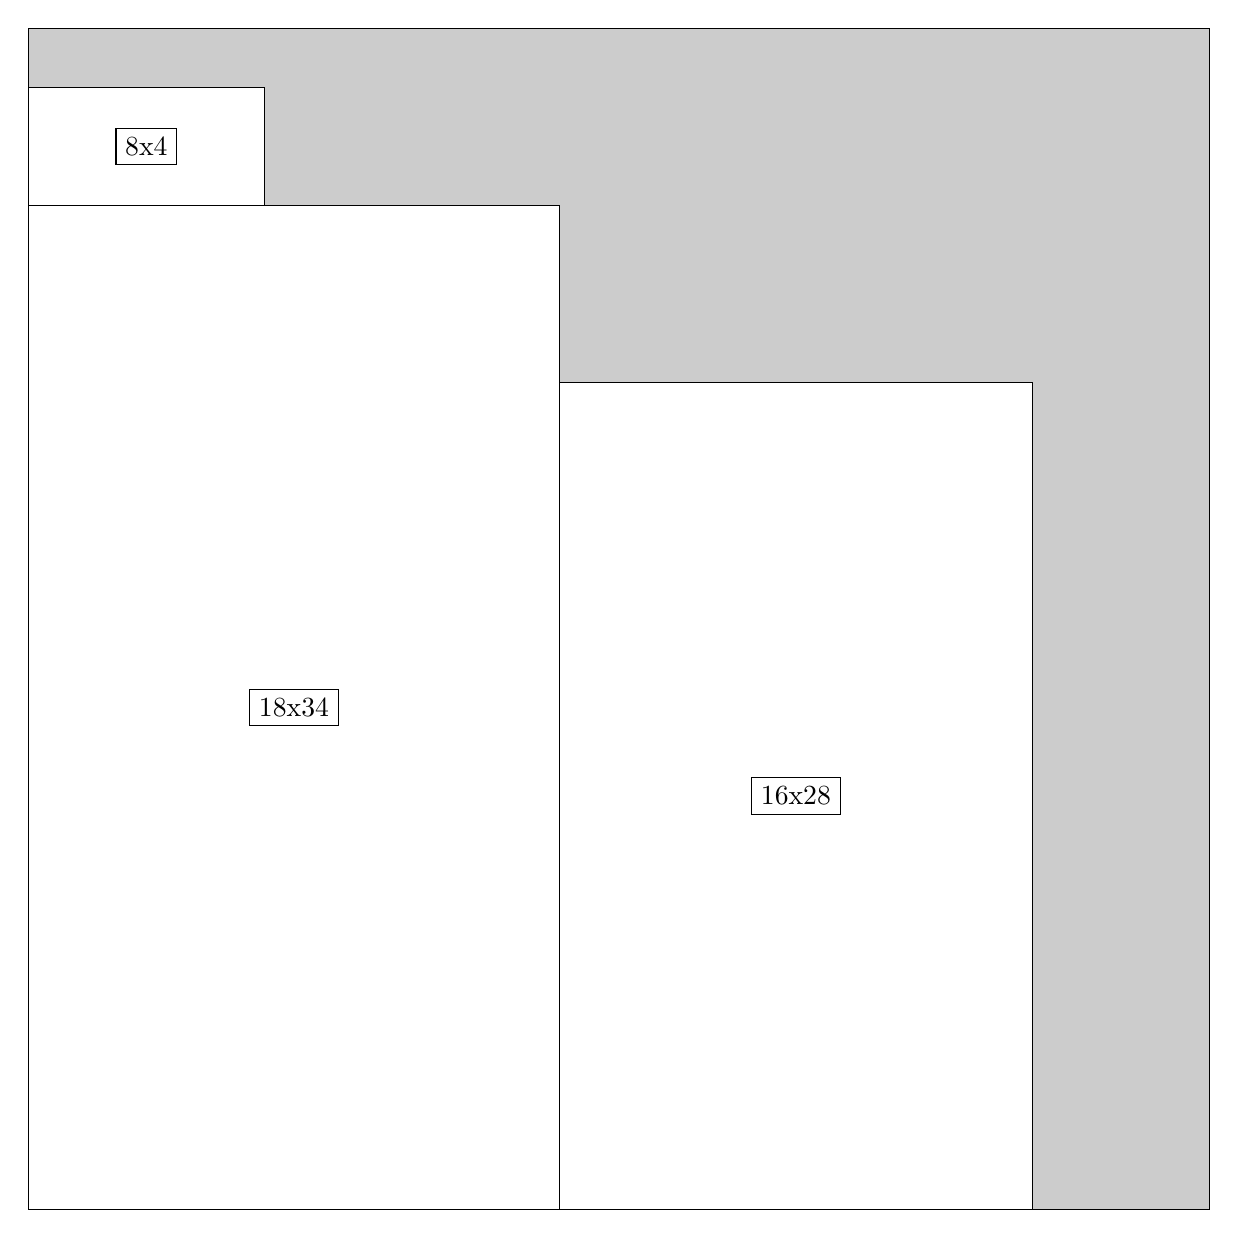
\begin{tikzpicture}[shorten >=1pt,scale=1.0,every node/.style={scale=1.0},->]
\tikzstyle{vertex}=[circle,fill=black!25,minimum size=14pt,inner sep=0pt]
\filldraw[fill=gray!40!white, draw=black] (0,0) rectangle (15.0,15.0);
\foreach \name/\x/\y/\w/\h in {18x34/0.0/0.0/6.75/12.75,16x28/6.75/0.0/6.0/10.5,8x4/0.0/12.75/3.0/1.5}
\filldraw[fill=white!40!white, draw=black] (\x,\y) rectangle node[draw] (\name) {\name} ++(\w,\h);
\end{tikzpicture}


w =18 , h =34 , x =0 , y =0 , v =612
\par
w =16 , h =28 , x =18 , y =0 , v =448
\par
w =8 , h =4 , x =0 , y =34 , v =32
\par
\newpage


\end{document}